\documentclass[a4paper]{book}

\usepackage{kotex}
\usepackage{setspace}
\usepackage{hyperref}
\usepackage{listings}
\usepackage[T1]{fontenc}   % Todo: because of double quotes in lstlisting 
\usepackage{multirow}
\lstset{
  basicstyle=\linespread{0.8}\selectfont,
  numbers=left,
  stepnumber=1
  }

\usepackage{tikz}
\usetikzlibrary{automata, positioning}

%%% Titles

\title{프로그램 분석 기초}
\author{최광훈}
% \institute{전남대학교}
\date{\today}

%%%

\doublespacing

\begin{document}

\maketitle

\tableofcontents

\chapter{프로그램 분석 개요}

\section{목적}

프로그램을 개발하거나 프로그램의 보안 취약점을 탐지할 때 다양한
프로그램 분석 방법을 사용하여 개발 생산성을 높이거나 꼼꼼하게 보안
취약점을 탐지하고 있다.
%
특정 프로그램 분석을 지원하는 오픈소스 소프트웨어도 다양하게 개발되어
개발자나 보안 담당자가 이러한 프로그램을 사용고 있다. 하지만 프로그램
분석에 대한 기초 지식이 없다면 이 프로그램을 제대로 사용하는데도
한계가 있다. 프로그램 분석에 대한 기초 지식을 갖추고 있다면 이러한
프로그램을 사용하는 것뿐만 아니라 자신의 목적에 맞추어 수정하는 것도
가능할 것이다.
%
하지만 프로그램 분석을 직접 배울곳이 마땅치 않고 프로그램 분석 기법과
밀접하게 관련된 프로그래밍언어론과 컴파일러를 공부할 수 있는 곳도
제한되어 있다. 설사 그러한 과목들을 배울 수 있다하더라도 프로그램 분석
기법을 배우는데 한계가 있다.

프로그램 분석은 어려운 주제이다. 여러 이유를 생각해볼 수 있다. 우선,
모든 프로그램 분석 기법은 복잡한 수학에 기반을 두고 있기
때문이다. 그리고, 분석 대상이 되는 프로그램을 작성한 프로그래밍언어
자체가 복잡하기 때문이다. 마지막으로 우리가 분석하고 싶은 품질 속성이
다양하기 때문이다.

프로그램 분석 기법을 쉽게 익힐 수 있도록 이 강의 노트를 구성하고자
한다. 우선, 수학을 사용하여 프로그램 분석을 설명하는 것을 최소한으로
제한하고 실행 가능한 명세를 통해서 설명한다. 그리고 간단한
프로그래밍언어 WHILE을 정의하여 이 언어로 작성된 프로그램을 대상으로
분석 기법을 설명한다. 마지막으로 어휘 분석, 구문 분석, 동적 의미, 타입
체킹, 정적 분석, 기호 실행으로 분석 기법을 한정하여 설명한다.

\section{미리 알아두면 좋을 내용}

프로그램 분석 기법에 대한 이 강의 노트를 공부하기 위해서 자료 구조와
기초 프로그래밍 지식이 필요하다. 리스트, 트리, 그래프와 같은 자료
구조를 이해하고 프로그래밍할 수 있어야 한다.

하스켈 프로그래밍언어로 프로그램 분석 기법에 대한 실행 가능한 명세를
작성한다. 이 언어를 사용한 이유는 수학 표기법을 사용하여 명세를 작성한
것에 비해 접근하기 쉽고, 하스켈 프로그램이 간결하여 명세로 삼기에
적합하기 때문이다. 표 \ref{table:lines}에 각 분석 방법과 그 방법을
구현한 하스켈 프로그램의 라인 수를 볼 수 있다. 88 라인에서 250
라인으로 여섯 가지 분석 방법을 작성하였다.

\begin{table}[ht]
\begin{center}
  \begin{tabular}{|c|c|}\hline
    분석 기법 명세 & 라인 \\\hline\hline
    어휘 분석 & 88 \\\hline
    구문 분석 & 228 \\\hline
    동적 의미 & 123 \\\hline
    정적 의미(타입 검사) & 145 \\\hline
    정적 분석 & 250 \\\hline
    기호 실행 & 208 \\\hline
  \end{tabular}
\end{center}
\caption{분석 방법과 하스켈로 작성한 실행 가능한 명세의 라인 수}
\label{table:lines}
\end{table}

하스켈 프로그래밍언어에 대한 공식 사이트는
\href{https://haskell.org}{https://haskell.org}이다. 다양한 레퍼런스를
이 웹 사이트에서 찾을 수 있다. 하스켈 기초 프로그래밍을 배우기 위해서
\href{https://haskell.mooc.fi/}{헬싱키 대학에서 만든 무크 사이트}를
이용할 수 있다. 이
\href{https://www.youtube.com/playlist?list=PLhbaMvGyp99_NphAX7k5OqcM1fXLZne8t}{무크
  사이트 내용으로 구성된 유튜브 동영상 강의}도 하스켈 프로그래밍을
배우기에 도움이 될 것이다.

여담이지만 하스켈과 같은 정통 함수형 프로그래밍언어를 한번 배우는 것은
설사 객체지향 프로그래밍언어를 주로 사용하는 사람들에게도 도움이 될
것이다.  최근 파이썬, C++, 자바, 자바스크립트, 코틀린, 스위프트와 같은
객체지향 프로그래밍언어에 람다, 다형 타입 (제네렉, 템플릿), 변경
불가능한 값(immutable value), 리스트 제시법(list comprehension)과 같은
함수형 프로그래밍언어의 핵심 특징들을 도입하고 있는 추세이다. 객체지향
프로그래밍 언어의 구문에 함수형 프로그래밍언어 특징을 구겨넣다보니
구문도 복잡하고 그 의미도 이해하기 어려운 경우도 있다.  정통 함수형
프로그래밍언어에서 그 특징들을 경험한다면 파이썬 프로그래밍을 할때도
프로그래밍에 대한 관점이 달라질 것이다.

이 외에 집합(set)이나 릴레이션(relation)과 같은 기초적인 수학 개념을
알 필요가 있다.

\section{이 강의 노트로 공부하는 방법}

이 강의 노트를 공부하는 방법은, 하스켈 프로그램으로 미리 준비해놓은
실행 가능한 명세들을 독자가 사용하는 프로그래밍언어로 다시
작성함으로써 각 분석 방법을 주체적으로 이해하는 방법을 권한다. 이 강의
노트에서는 파이썬을 선택하여 설명한다. 

강의 노트에서 사용하는 하스켈 프로그램의 내용은 다음과 같다.

\begin{itemize}
\item \href{https://github.com/kwanghoon/Lecture_SAV/tree/master/whilelang/example}{WHILE 프로그래밍 언어 예제 프로그램}
\item \href{https://github.com/kwanghoon/Lecture_SAV/blob/master/whilelang/app/Lexer.hs}{어휘 분석(lexical analyzier)}
\item \href{https://github.com/kwanghoon/Lecture_SAV/blob/master/whilelang/app/Parser.hs}{구문 구조 분석(Parser)}
\item \href{https://github.com/kwanghoon/Lecture_SAV/blob/master/whilelang/app/interp/Interp.hs}{동적 의미(semantics)}
\item \href{https://github.com/kwanghoon/Lecture_SAV/blob/master/whilelang/app/typecheck/Typecheck.hs}{정적 의미-타입체킹}
\item \href{https://github.com/kwanghoon/Lecture_SAV/blob/master/whilelang/app/dataflow/Dataflow.hs}{정적 분석-자료 흐름 분석}
\item \href{https://github.com/kwanghoon/Lecture_SAV/blob/master/whilelang/app/symexec/SymExec.hs}{기호 실행}
\end{itemize}

이 프로그램을 \href{https://github.com/kwanghoon/Lecture_SAV}{깃허브
  저장소}에서 내려 받고,
%
빌드한다.

기본적으로
\href{https://docs.haskellstack.org/en/stable/install_and_upgrade/}{하스켈
  빌드 시스템 도구 스택(stack)}을 설치해야 한다.
%
추가로 기호 실행 분석에서 사용하는 산술 복합 논리식을 해결하는 풀이
엔진 (SMT -Satisfiability Module Theories - solver) Z3 라이브러리가
필요하다.

\begin{itemize}
\item 리눅스
\begin{verbatim}
$ sudo apt-get install libz3-dev
$ git clone https://github.com/kwanghoon/Lecture_SAV
$ cd Lecture_SAV/whilelang
$ stack build
\end{verbatim}
\item 윈도우즈
  \begin{itemize}
  \item \href{https://github.com/Z3Prover/z3/releases/tag/z3-4.8.12}{z3-4.8.12 버전}을 내려받기
  \item 
  \begin{verbatim}
  (D:\z3-4.8.12-x64-win 디렉토리 아래 bin에 라이브러리, include에 헤더 파일이 있다고 가정)
    D:\> git clone https://github.com/kwanghoon/Lecture_SAV
    D:\> cd Lecture_SAV/whilelang
    D:\> stack build 
           --extra-include-dirs=D:\z3-4.8.12-x64-win\include
           --extra-lib-dirs=D:\z3-4.8.12-x64-win\bin
  \end{verbatim}
  \end{itemize}
\end{itemize}

하스켈 프로그램을 빌드한 다음 어휘 분석부터 기호 실행까지 실행하는
방법은 다음과 같다. 실행 파일을 통해 각 분석 방법을 다음과 같이 실행할
수 있다.

\begin{verbatim}
$ stack exec -- whilelang-exe --lex ./example/while2.while
$ stack exec -- whilelang-exe --parse ./example/while2.while
$ stack exec -- whilelang-exe --typecheck ./example/while2.while
$ stack exec -- whilelang-exe --dataflow ./example/while2.while
$ stack exec -- whilelang-exe --symexec ./example/while2.while
\end{verbatim}

하스켈 프로그램을 read-eval-print 방식으로 실행할 수도 있다. 

\begin{verbatim}
$ stack ghci --
ghic> let srcFile = "./example/while2.while"
ghci> doLexing srcFile
ghci> doParsing srcFile
ghci> doRun srcFile
ghci> doTypecheck srcFile
ghci> doAnalysis srcFile
ghci> doSymbolic srcFile
\end{verbatim}

WHILE 프로그램을 하스켈 어휘 분석과 구문 구조 분석 결과로 얻은 추상
구문 트리(AST, Abstract Syntax Tree)를 다른 프로그래밍언어에서
사용하기 위해서 이 트리를 JSON 형식으로 출력하는 방법을 제공한다.

\begin{verbatim}
$ stack exec -- whilelang-exe --json ./example/while2.while
\end{verbatim}

\begin{verbatim}
$ stack ghci --
ghic> let srcFile = "./example/while2.while"
ghci> doJson srcFile
\end{verbatim}

파이썬 프로그램에서 이 JSON 형식의 분석 내용을 읽어서 원하는 분석을
진행할 수 있다.

\chapter{WHILE 프로그래밍언어}

프로그램 분석 대상으로 C나 Java와 같은 프로그래밍언어를 사용하면 그
언어의 복잡성으로 프로그램 분석을 집중해서 설명하기 어려울 수 있다.
그러한 이유로 기초적인 특징만을 고려한 프로그래밍언어를 선택하고 그
언어로 작성한 프로그램들을 대상으로 한다. 이 강의노트에서 WHILE
프로그래밍 언어를 선택했다.

\section{WHILE 프로그래밍 언어 구문  개요}

WHILE 언어는 가장 기초적인 특징들로만으로 구성되어 있다. 문장으로
할당문, 조건문, WHILE 반복문, 복합문 (여러 문장들을 세미콜론으로
분류하여 나열), 생략문(SKIP), 입출력문, assert문이 있다. 문장내에
사용할 수 있는 식의 종류는 상수, 변수, 단항 연산과 이항 연산이
있다. 정수와 부울, 두 가지 종류의 값을 사용하며, 사칙연산과 나머지
연산, 비교 연산 두 종류(\textless, ==)와 논리곱, 논리합, 논리 부정
연산이 있다.

WHILE 프로그램은 변수 타입들을 먼저 선언하고 뒤이어 문장들이 나오도록
구성되어 있다. 함수나 클래스는 제공하지 않는다.

정수를 입력받아 변수 x에 놓고 팩토리얼을 구해 출력하는 WHILE 에제
프로그램을 살펴보자. 변수 x와 z를 정수 타입으로 선언한다. 정수를 입력
받아 변수 x에 놓고, 변수 z는 1로 초기화한다. WHILE 반복문으로, 변수
x를 1씩 감소시키며 변수 z에 누적해서 변수 x를 곱하는 것을 변수 x의
값이 1보다 큰 동안 반복한다. 마지막으로 변수 z의 값을 출력한다.

\begin{figure}[ht]
\begin{center}
\begin{minipage}[h]{.4\textwidth}
\begin{lstlisting}
int x;
int z;

read(x);

z = 1;
while (x > 1)
 {
   z = z * x;
   x = x - 1
 };

write(z)
\end{lstlisting}
\end{minipage}
\end{center}
\caption{팩토리얼 프로그램}
\label{fig:factorial}
\end{figure}

더 많은 WHILE 프로그램 예제는
\href{https://github.com/kwanghoon/Lecture_SAV/tree/master/whilelang/example}{강의
  웹 사이트}에서 확인할 수 있다.

\section{WHILE 프로그램을 자료구조로 표현: 추상구문트리}

이제 WHILE 프로그램을 자료구조로 표현하는 방법을 살펴보자. 일반적으로
프로그램에 분석 방법을 적용하려면 이 프로그램 텍스트를 먼저
추상구문트리(Abstrac Syntax Tree, AST)로 표현하는 과정이 선행되어야
한다. 추상구문트리는 프로그램의 구조를 모두 담고 있는 트리 자료
구조이다.

WHILE 프로그램의 추상구문트리를 다음과 같은 하스켈 프로그램의 타입
선언으로 그 명세를 작성하려고 한다.

2번째 줄 data Prog에서 data는 새로운 타입을 정의하는 하스켈 키워드이고
뒤이어 나오는 Prog는 이때 정의하는 타입 이름이다.

WHILE 프로그램은 이 Prog 타입의 값으로 표현하려 한다. 뒤이어 Prog
Decls Comms에서 동일한 이름이어서 혼동되지만 이때 Prog는 이 값에
붙이는 태그로 이해할 수 있다.  이 태그가 붙은 값은 Decls 타입의 값과
Comms 타입의 값이 뒤따라야만 비로서 Prog 타입의 값이 완성된다.

4번째 줄 type Decls에서 type은 새로운 타입 이름을 붙이는 하스켈
키워드이고 뒤이어 나오는 Decls는 이때 새로 붙이려는 타입 이름이다.
하스켈에서 리스트 타입은 [ - ] 대괄호를 사용한다. 그 안에 리스트
원소의 타입을 넣는다. 즉, [ Decl ]은 Decl 타입의 값을 원소로 하는
리스트의 타입을 뜻한다. 이 [ Decl ] 타입을 반복해서 나중에 언급해도
되나 짧게 Decls 타입이라 부르겠다는 것이 4번째 줄의 새로운 타입 이름
붙이기 선언이 의도하는 바이다.

이 Decls 타입으로 WHILE 프로그램의 선언들을 표현하려 한다. Decls
타입은 Decl 타입을 원소로 하는 리스트 타입인데, Decl 타입은 7번째 줄에
Type 타입과 VarName 타입의 쌍 타입으로 정의되어 잇다.

Type 타입은 WHILE에서 사용하는 정수 타입과 부울 타입을 표현한다.
10번째 줄에 data Type을 선언하였고, 이때 두 가지 타입을 구분해서
표현하도록 각각 TyInt와 TyBool 두 종류의 태그를 도입했다. 두 태그
사이의 바($|$)는 Type 타입의 값이 TyInt이거나 또는 TyBool 둘 중 하나를
선택 가능한 것임을 나타낸다.

예를 들어, ``int x'' 타입 선언을 표현한 하스켈 값은 Decls 타입의
\begin{center}
  [ (TyInt, ``x'') ]
\end{center}
이다.


VarName 타입은 변수 이름을 표현하는 타입으로 14번째 줄에 하스켈 문자열
타입인 String으로 정의되어 있다.

2번째 줄 Prog Decls Comms에서 Comms 타입으로 WHILE 프로그램 변수
선언에 뒤따라 나오는 문장들을 표현하려 한다.

5번째 줄 type Comms 선언도 4번째 줄과 같이 이해할 수 있다. Comm 타입은
17번째 줄에 선언한 WHILE 언어에서 허용하는 문장들을 모아놓은 타입이다.
8가지 문장 종류를 구분하기 위해 CSkip, CSeq, CAssign, CRead, CWrite,
CIf, CWhile, CAssert 8가지 태그를 도입하였다.

CSkip 태그는 뒤이어 채워야할 값이 없지만, CAssign 태그는 VarName
타입의 값과 Expr 타입의 값이 함께 와야 비로서 Comm 타입의 완전한
문장이 된다.

예를 들어, 할당문 ``x = 0''을 표현한 하스켈 값은 Comm 타입의 
\begin{center}
  CAssign ``x'' (ECst (CInt 0))
\end{center}
이다. 하스켈의 String 타입의 문자열 ``x''는 VarName 타입의 값이기도
하다. 28-29번째 줄을 보면 data Expr 선언으로 WHILE 언어의 식을 선언한
타입이 있는데, 이 중 상수식을 표현하는 태그가 ECst이다. ECst 태그를
식으로 완성하기 위해서 Const 타입의 값이 필요한데, 34-36번째 줄에 data
Const 선언으로 이 타입이 선언되어 있다. 35번째 줄에 CInt 태그와 하스켈 정수 타입 Int로 WHILE 언어의 정수 값을 표현한다.

또 다른 할당문 예를 살펴보자. ``x = x + 1''은 변수 x의 값을 1 증가시키는 할당문이다. 이를 표현한 하스켈 값은 Comm 타입의 
\begin{center}
  CAssign ``x'' (EBinOp OpAdd (EVar "x") (ECst (CInt 1)))
\end{center}
이다. WHILE 언어의 식을 표현하는 Expr 타입(28-32번째줄)을 보면 이
할당문의 오른쪽 식에서 사용한 이진 연산 덧셈은 EBinOp OpAdd $\cdots
\ \cdots$의 구조로 표현한다. 이때 OpAdd는 Op 타입의 가능한 값 중
하나로 38-48번째 줄에 data Op 선언에서 39번째 줄에 있다.

뒤이어 덧셈의 두 피연산자 ``x''와 ``1''에 해당하는 식이 나온다. 변수
x는 Expr 타입의 EVar 태그를 사용하여 EVar ``x''로 표현하고, 상수 1은
Expr 타입의 ECst 태그를 사용하여 ECst (CInt 1)로 작성한다. 이때 Const
타입의 정수를 나타내는 CInt 태그와 하스켈 정수 값 1로 표현한다.

지금까지 설명을 종합하면, 변수 x를 선언하고, 0으로 초기화하고, 1 증가시키는 WHILE 프로그램을 하스켈로 표현하면 다음과 같다.

{\footnotesize
 \begin{minipage}[h]{0.15\textwidth}
\begin{verbatim}
int x;
x = 0;
x = x + 1
\end{verbatim}
\end{minipage}
$\ \ \Rightarrow \ \ $
\begin{minipage}[h]{0.6\textwidth}
\begin{verbatim}
Prog
 [(TyInt,"x")]
 [ CAssign "x" (ECst (CInt 0)),
   CAssign "x" (EBinOp OpAdd (EVar "x") (ECst (CInt 1))) ]
\end{verbatim}
\end{minipage}
}

\begin{figure}[h]
{\footnotesize
\begin{center}
\begin{minipage}[h]{.6\textwidth}
\begin{lstlisting}[language=Haskell]
-- Program
data Prog = Prog Decls Comms

type Decls = [ Decl ]
type Comms = [ Comm ]

type Decl  = (Type, VarName)

-- Type
data Type =
    TyInt
  | TyBool

type VarName  = String

-- Statement
data Comm =
    CSkip
  | CSeq Comm Comm
  | CAssign VarName Expr
  | CRead VarName
  | CWrite Expr
  | CIf Expr Comm Comm
  | CWhile Expr Comm
  | CAssert Expr

-- Expression
data Expr =
    ECst   Const
  | EVar   VarName
  | EBinOp Op Expr Expr
  | EUnaryOp Op Expr

data Const =
    CInt  Int
  | CBool Bool

data Op =
    OpAdd
  | OpSub
  | OpMul
  | OpDiv
  | OpMod
  | OpLessThan   -- x < y
  | OpEqual      -- x == y
  | OpAnd
  | OpOr
  | OpNot
\end{lstlisting}
\end{minipage}
\end{center}
}
\caption{WHILE 프로그래밍 언어의 추상 구문 트리 정의 (하스켈로 작성한 명세)}
\label{fig:haskellastdatatype}
\end{figure}

%% ghci> :type ECst
%% ECst :: Const -> Expr
%% ghci> ECst (CInt (-126))
%% ECst (CInt (-126))
%% ghci> if x > y then x = 0 else y = 0 

%% <interactive>:3:17: error: parse error on input ‘=’
%% ghci> CIf (EUnaryOp OpNot (EBinOp OpOr (EBinOp OpLessThan (EVar "x") (Evar "y") ) (EBinOp OpEqual (EVar "x") (EVar "y") )  ))

%% <interactive>:4:65: error:
%%     • Data constructor not in scope: Evar :: String -> Expr
%%     • Perhaps you meant ‘EVar’ (imported from Expr)
%% ghci> CIf (EUnaryOp OpNot (EBinOp OpOr (EBinOp OpLessThan (EVar "x") (EVar "y") ) (EBinOp OpEqual (EVar "x") (EVar "y") )  ))

%% <interactive>:5:1: error:
%%     • No instance for (Show (Comm -> Comm -> Comm))
%%         arising from a use of ‘print’
%%         (maybe you haven't applied a function to enough arguments?)
%%     • In a stmt of an interactive GHCi command: print it
%% ghci> CIf (EUnaryOp OpNot (EBinOp OpOr (EBinOp OpLessThan (EVar "x") (EVar "y") ) (EBinOp OpEqual (EVar "x") (EVar "y") )  ))  (CAssign "x" (Const (CInt 0))) (CAssign "y" (Const (CInt 0)))

%% <interactive>:6:136: error:
%%     • Data constructor not in scope: Const :: Const -> Expr
%%     • Perhaps you meant variable ‘const’ (imported from Prelude)

%% <interactive>:6:167: error:
%%     • Data constructor not in scope: Const :: Const -> Expr
%%     • Perhaps you meant variable ‘const’ (imported from Prelude)
%% ghci> CIf (EUnaryOp OpNot (EBinOp OpOr (EBinOp OpLessThan (EVar "x") (EVar "y") ) (EBinOp OpEqual (EVar "x") (EVar "y") )  ))  (CAssign "x" (ECst (CInt 0))) (CAssign "y" (ECst (CInt 0)))
%% CIf (EUnaryOp OpNot (EBinOp OpOr (EBinOp OpLessThan (EVar "x") (EVar "y")) (EBinOp OpEqual (EVar "x") (EVar "y")))) (CAssign "x" (ECst (CInt 0))) (CAssign "y" (ECst (CInt 0)))
%% ghci> let thenComm = (CAssign "x" (ECst (CInt 0)))
%% ghci> let elseComm = (CAssign "y" (ECst (CInt 0)))
%% ghci> let cond = (EUnaryOp OpNot (EBinOp OpOr (EBinOp OpLessThan (EVar "x") (EVar "y")) (EBinOp OpEqual (EVar "x") (EVar "y"))))
%% ghci> CIf cond thenComm elseComm
%% CIf (EUnaryOp OpNot (EBinOp OpOr (EBinOp OpLessThan (EVar "x") (EVar "y")) (EBinOp OpEqual (EVar "x") (EVar "y")))) (CAssign "x" (ECst (CInt 0))) (CAssign "y" (ECst (CInt 0)))
%% ghci>

\section{파이썬 구현}

WHILE 프로그램의 추상구문트리를 표현하는 명세로 하스켈 타입을
선언하였다. 이 명세에서 의도하는 바를 파이썬으로 구현해본다.

type T = ... 또는 data T = ... 형태로 선언한 하스켈 타입은 파이썬
클래스로 옮길 수 있다.

예를 들어, data Prog 선언은 Prog라는 이름을 갖는 클래스를 도입하고 그
안에 Prog Decls Comms에서 필요한 Decls를 저장하는 멤버 변수와 Comms를
저장하는 멤버 변수를 두는 형태로 파이썬 클래스를 구현할 수 있다.

type Decls 선언은 Decls라는 이름의 파이썬 클래스를 선언하고 멤버
변수로 Decl 값의 리스트에 해당하는 파이썬 리스트 값을 저장할 수 있도록
구성하면 된다.

data Comm 선언은 8가지 서로 다른 태그가 있다. 이러한 형태의 명세는
Comm 이라는 이름의 기반 클래스를 먼저 선언한다. 멤버 변수는 특별히
필요하지 않다. 각 태그에 대해 클래스를 도입하되 이 클래스는 기반
클래스를 상속 받도록 서브 클래스로 구성한다. 각 태그에 수반해야할 값들
(예를 들어 CSeq의 경우 두 개의 Comm 타입의 값들이 필요하다다)을 서브
클래스의 멤버 변수로 두어 하스켈 명세를 충실히 구현할 수 있다.


\chapter{구문 분석(Syntactic analysis)}

먼저 언어(languages), 문법(grammar), 오토마타(automata)의 3가지 기초
개념을 소개하고, 이를 바탕으로 어휘 분석(lexical anlaysis)과 구문 구조
분석(parsing)을 설명한다.

\begin{table}[ht]
\begin{center}
\begin{tabular}{|c|l|} \hline
  \multirow{2}{*}{공통 주제}
    & 오토마타, 문법, 언어 \\ \cline{2-2}
    & 촘스키 계층 \\ \hline
  \multirow{3}{*}{어휘 분석} & 유한 오토마타 \\ \cline{2-2}
    & 정규식 \\ \cline{2-2}
    & 어휘 분석기 구조 \\ \hline
  \multirow{5}{*}{구문 구조 분석}
    & LR 파싱 \\ \cline{2-2}
    & LR 구문 분석기 구조 \\ \cline{2-2}
    & LR 문법 작성 요령 \\ \cline{2-2}
    & 모호한 문법 처리 \\ \cline{2-2}
    & 에러 복구 \\ \hline
\end{tabular}
\caption{기본 개념과 구문 분석 주제}
\label{table:syntaxanalysis}
\end{center}
\end{table}


\section{기본 개념: 언어, 문법, 오토마타}


구문 분석에서 사용하는 3가지 기본 개념은 언어, 문법, 오토마타이다. 이
장에서 이 개념들이 무엇이고 서로 어떻게 연결되어 있는지에 대해 살펴본다.

\subsection{언어}
\label{subsec:language}


우리말이나 영어와 같은 자연어(natural languages)를 익숙하게 사용하고
있지만 아마도 언어(langauges)가 무엇인지 설명하기는 쉽지 않을 것이다.

언어는 단어(word) 또는 문장(sentence)들의 집합으로 정의한다. 언어의
예로, 영문자로 시작하고 뒤이어 영문자나
숫자가 반복되는 간단한 형태의 변수 이름 또는 함수 이름과 같은
식별자들(identifier)의 집합을 고려해볼 수 있다.
%
편의상 소문자 영문자만 고려한다. 그러한 식별자들을 모두 나열한 집합을
언어로 정의할 수 있다. 물론 그 식별자의 수는 무한하다.

\begin{center}
  \{ \ a, ... ,z, aa, ..., az, a0, ..., a9,
       ba, ..., bz, b0, ..., b9, ca, ...
     \ 
  \}
\end{center}

편의상 이 언어에 $\L_{id}$이라는 이름을 붙이자. $\L_{id}$로 x나 y가
가능하고, varname과 obj123을 사용할 수 있다. str2int와 같이 다소
낯설수 있지만 숫자가 중간에 놓인 단어도 가능하다.

각 단어나 문장을 구성하는 요소는 $\L_{id}$에서 영문자와 숫자이다.
\begin{center}
  \{ \ a, ... ,z, 0, ..., 9
     \ 
  \}
\end{center}


이와 같은 단어 또는 문장의 구성 요소를 알파벳(alphabet)이라
부른다. 영어에서는 알파벳이 에이부터 제트까지이지만 여기서
이야기하려는 알파벳은 영문자 뿐만 아니라 점, 세미콜론, 따옴표를 포함한
임의의 기호로 구성될 수 있다. 알파벳을 그리스 문자 $\Sigma$로
표현한다.

단어 또는 문장은 이 알파벳을 구성하는 기호들을 이어 붙여(concatenate)
구성하고, 원하는 형태의 단어 또는 문장들을 모아 집합으로 구성하여
언어를 이룬다. 예를 들어, $L_{id}$의 단어 str2int는 $\Sigma_{id}$에서
s, t, r, 2, i, n, t를 꺼내 차례로 붙여 구성한 것이다. 이때 기호 t를 두
번 사용하였다.

원하는 단어를 구성하기 위해서 동일한 기호를 되풀이해서 사용할 수
있다. $\Sigma^i$는 알파벳에 윗 첨자 $i$를 붙여 알파벳에서 $i$번
반복해서 기호를 꺼내 붙여만든 모든 단어들의 집합이다. $\Sigma^1$에
x나 y가 포함되어 있고, str2int는 $\Sigma^7$의 원소이다.

$\Sigma^0$는 전혀 기호를 꺼내지 않았으니 비어있는 단어로만 되어 있는
집합이다.  보통 비어있는 단어를 $\epsilon$으로 표시한다. 즉, $\Sigma^0
\ = \ \{ \ \epsilon \ \}$. 어떤 언어에서 비어 있는 단어를 허용할지
여부는 그 언어를 설계하는 사람의 의도에 달려 있다.

이와 같이 언어를 알파벳을 임의의 횟수로 조합해서($\Sigma^*$) 구성한
모든 가능한 단어나 문장들로 이루어진 전체 집합의 일부분으로 정의할 수
있다.

\begin{center}
  $L \ \subseteq \ \Sigma^0 \cup \Sigma^1 \cup \Sigma^2 \cup \cdots  \ = \ \Sigma^*$
\end{center}

\subsection{문법}
\label{subsec:grammar}


언어를 분석하기 위해 이 언어를 표현하는 방법이
필요하다. 문법(Grammar)은 언어를 기술하는 다양한 방법 중에 널리
사용되는 방법이다. 자연어의 문법을 먼저 살펴보면, 영어 문법을 통해
특정 문장이 잘 구성되었는지 여부를 가릴 수 있다. 주어 다음에 동사가
나오고 타동사의 경우 목적어가 순서대로 나오는 식이다. 이와 같이
문법에는 주어, 동사, 목적어와 같은 구성 요소가 있고 어떻게
구성해야하는지 정하는 규칙이 있다.

\begin{center}
  \textless sentence\textgreater
  \ $\rightarrow$ \ 
  \textless subject\textgreater \ 
  \textless verb\textgreater \ 
  \textless object\textgreater
\end{center}

프로그래밍언어와 같은 형식 언어(formal languages)에서도 비슷한 형태의
규칙으로 문법을 기술한다. 이 규칙을 생산(production)이라
부른다.
%
자연어 문법의 규칙을 사용하여 \textless sentence\textgreater를
\textless subject\textgreater \ \textless verb\textgreater \ \textless
object\textgreater로 펼쳐서 주어, 동사, 목적어 순서대로 유효한 문장을
만든다.
%  
형식언어의 생산 규칙도 어떤 기호들을 다른 기호들로 대체하면서 유효한
문장을 만든다.
%
예를 들어, 식별자 언어 $\L_{id}$에 포함된 단어만 만드는 문법($G_{id}$)의 생산
규칙($P_{id}$)을 다음과 작성해 볼 수 있다.
\begin{center}
  $S_{id} \ \rightarrow \ a \ AlphaNum$ \\
  ... \\
  $S_{id} \ \rightarrow \ z \ AlphaNum$ \\
  $S_{id} \ \rightarrow \ 0 \ AlphaNum$ \\
  ... \\
  $S_{id} \ \rightarrow \ 9 \ AlphaNum$ \\
  $AlphaNum \ \rightarrow \ AlphaNum \ a$ \\
  ... \\
  $AlphaNum \ \rightarrow \ AlphaNum \ z$ \\
  $AlphaNum \ \rightarrow \ AlphaNum \ 0$ \\
  ... \\
  $AlphaNum \ \rightarrow \ AlphaNum \ 9$ \\
  $AlphaNum \ \rightarrow \ $
\end{center}


문법에서 다루는 기호는 두 가지, 단말 기호(terminals)와 비단말
기호(nonterminals)가 있다.  생산 규칙의 왼쪽에 나타나서 다른 기호들로
대체할 수 있는 기호를 비단말 기호라 하고, 그렇지 않고 더이상 대체되지
않는 기호를 단말 기호라 부른다.  예제 문법에서 S와 AlphaNum은 비단말
기호들이고 a부터 z와 0부터 9를 단말 기호들이다.

위 문법을 사용해서 단어 str2int를 만들어보자. 문법에서 시작 기호(start
symbol)에서부터 생산 규칙을 사용해 왼쪽 비단말 기호를 오른쪽 기호들로
대체하면서 단어를 만든다. 예제 문법에서 S를 시작 기호로 정한다.

\begin{center}
  \begin{tabular}{r c l l }
    $S_{id}$
      & $\Rightarrow$ & $s \ AlphaNum$  & by $S_{id} \ \rightarrow \ s \ AlphaNum$ \\
      & $\Rightarrow$ & $s \ AlphaNum \ t$ & by $AlphaNum \ \rightarrow \ AlphaNum \ t$ \\
      & $\Rightarrow$ & $s \ AlphaNum \ n \ t$ & by $AlphaNum \ \rightarrow \ AlphaNum \ n$ \\
      & $\Rightarrow$ & $s \ AlphaNum \ i \ n \ t$ & by $AlphaNum \ \rightarrow \ AlphaNum \ i$ \\
      & $\Rightarrow$ & $s \ AlphaNum \ 2 \ i \ n \ t$ & by $AlphaNum \ \rightarrow AlphaNum \ 2$ \\
      & $\Rightarrow$ & $s \ AlphaNum \ r \ 2 \ i \ n \ t$ & by $AlphaNum \ \rightarrow \ AlphaNum \ r$ \\
      & $\Rightarrow$ & $s \ AlphaNum \ t r 2 \ i \ n \ t$ & by $AlphaNum \ \rightarrow \ AlphaNum \ t$ \\
      & $\Rightarrow$ & $s \ t \ r \ 2 \ i \ n \ t$ & by $AlphaNum \ \rightarrow \ $ 
  \end{tabular}
\end{center}

일반적으로 문법 $G$는 단말(V)과 비단말 기호(T), 시작 비단말 기호(S),
생산 규칙(P)로 구성된다.

\begin{center}
  $ G \ = \ (V, T, S, P) $
\end{center}

예제를 통해 살펴본 바와 같이, 식별자를 만드는 문법 $G_{id}$는 다음과 같다.

\begin{center}
  $ G_{id} \ = \ (\{S, AlphaNum\}, \ \{a,...,z,0,...9 \}, \ S_{id}, \ P_{id}) $
\end{center}

과연 이 문법 $G_{id}$로 만들 수 있는 모든 단어들을 모으면, $
L(G_{id})$, 식별자 언어 $L_{id}$와 동일할까?
%
즉, 이 문법으로 단어를 만들면 그 단어는 식별자 언어에 항상 포함되고,
식별자 언어에서 단어를 뽑으면 이 문법으로 그 단어를 항상 만들수
있는지? 답은 그렇다이다.

\begin{equation}
  L(G_{id}) \ = \ L_{id}
  \label{equ:gidisequaltolid}
\end{equation}

식별자 언어와 문법의 경우는 동일하다. 여기에서 논의하지 않지만 증명도
가능하다. 일반적으로 언어와 문법이 동일한지를 보이기 어렵다.


식별자 문법에서 사용한 생산 규칙은 화살표 왼쪽은 비단말 기호가 한 개
나타나고 오른쪽은 비단말 기호를 최대 한 개 사용하고 단말 기호는
제한없이 사용할 수 있는 제한적인 형태를 가지고 있었다. 이러한 형태의
생산 규칙으로 이루어진 문법을 선형 문법(Linear grammar)라
부른다.

$G_{id}$의 생산 규칙을 다음과 같이 변경해도
\begin{center}
  ... \\
  $AlphaNum \ \rightarrow \ a \ AlaphaNum$,\\
  ...,\\
  $AlphaNum \ \rightarrow \ z \ AlaphaNum$, \\
  $AlphaNum \ \rightarrow \ 0 \ AlaphaNum$, \\
  ..., \\
  $AlphaNum \ \rightarrow \ 9 \ AlaphaNum$ \\
  ...
\end{center}
$L(G_{id})$ 와 동일한 언어를 생성하는 문법이다. 이 생산규칙은 오른편의
비단말 기호의 위치가 모두 단말 기호의 오른편에 있는 형태로 선형
문법보다 더 제한적이다. 이러한 형태의 생산 규칙만을 가지고 있으면 정규
문법(Regular grammar)이라 부른다.

아래 예시는 오른편에 비단말 기호가 한 개 이상 나타난 생산 규칙을
가지고 있어 정규 문법이나 선형 문법보다 자유로운 형태이다.
\begin{center}
  $S \ \rightarrow \ A \ S \ B$ \\
  $S \ \rightarrow \ $ \\
  $A \ \rightarrow \ a$ \\
  $B \ \rightarrow \ b$
\end{center}
이 문법으로 생성하는 언어는 $L(S) = \{ \ a^n b^n \ | \ n \geq 0
\ \}$이다. 자유 문맥 문법(Context-free grammar)이라 부른다.  생산
규칙의 왼쪽 비단말 기호가 나타나면 그 주변 문맥을 고려하지 않고 그
규칙을 적용할 수 있다.

문맥에 민감한 문법(Context-sensitive grammar)은 주변 문맥을 고려해서
생산 규칙을 적용하도록 작성한 문법이다. 예를 들어 $L(S) = \{ \ a^n b^n
c^n \ | \ n \geq 1 \ \}$의 문법은 다음과 같다.

\begin{center}
  $S \ \rightarrow \ a \ b \ c \ | \ a \ A \ b \ c$ \\
  $A \ b \ \rightarrow \ b \ A$ \\
  $A \ c \ \rightarrow \ B \ b \ c \ c$ \\
  $a \ B \ \rightarrow \ a \ a \ | \ a \ a \ A$
\end{center}

이 문법으로 $a^3 b^3 c^3$를 유도해보자\footnote{Peter Linz, Introduction to Formal Languages and Automata, Example 11.2 in Chapter 11.3.}.

\begin{center}
  \begin{tabular}{r c l l }
    $S$
      & $\Rightarrow$ & $a \ A \ b \ c$  & by $S \ \rightarrow \ a \ A \ b \ c$ \\
      & $\Rightarrow$ & $a \ b \ A \ c$ & by $A \ b \ \rightarrow \ b \ A$ \\
      & $\Rightarrow$ & $a \ b \ B \ b \ c \ c$ & by $A \ c \ \rightarrow \ B \ b \ c \ c$ \\
      & $\Rightarrow$ & $a \ B \ b \ b \ c \ c$ & by $b \ B \ \rightarrow \ B \ b$ \\
      & $\Rightarrow$ & $a \ a \ A \ b \ b \ c \ c$ & by $a \ B \ \rightarrow \ a \ a \ A$ \\
      & $\Rightarrow$ & $a \ a \ b \ A \ b \ c \ c$ & by $A \ b \ \rightarrow \ b \ A$ \\
      & $\Rightarrow$ & $a \ a \ b \ b \ A \ c \ c$ & by $A \ b \ \rightarrow \ b \ A$ \\
      & $\Rightarrow$ & $a \ a \ b \ b \ B \ b \ c \ c \ c$ & by $A \ c \ \rightarrow \ B \ b \ c \ c$ \\
      & $\Rightarrow$ & $a \ a \ b \ B \ b \ b \ c \ c \ c$ & by $b \ B \ \rightarrow \ B \ b$ \\
      & $\Rightarrow$ & $a \ a \ B \ b \ b \ b \ c \ c \ c$ & by $b \ B \ \rightarrow \ B \ b$ \\
      & $\Rightarrow$ & $a \ a \ a \ b \ b \ b \ c \ c \ c$ & by $a \ B \ \rightarrow \ a \ a$
  \end{tabular}
\end{center}

정규 문법, 선형 문법, 문맥 자유 문법, 문맥에 민간함 문법은 생산 규칙의
형태에 따라 해당 클래스의 이름을 붙였다.  하지만 구문 구조 분석에서
소개할 LR 문법의 경우 생산 규칙의 형태로 그 문법의 특징을 규정 짓기
어려워서 그 문법으로 생산하는 단어를 받아들이는 일종의 컴퓨터 또는
기계에 해당하는 오토마톤이 존재하는지 여부로 그 클래스를 정의하는
경우도 있다. 그 존재 여부는 LR 문법으로부터 LR 오토마톤을 만드는
알고리즘으로 판단한다.


\subsection{오토마타}
\label{subsec:automata}

오토마타(automata)\footnote{또는 오토마톤(automaton)}는 컴퓨터의 상태
전이 요소를 강조하여 추상화한 모델이다. 컴퓨터는 입출력, 기억 장치,
제어부로 구성한다. 마찬가지로 오토마타도 기억 장치의 상태와 입력을
받아 다음 기억 장치의 상태와 출력을 내는 전이 함수(Transition
function)로 정의한다. 이 함수가 일종의 제어부에 해당한다.

기억 장치의 형태에 따라 다양한 클래스의 오토마타를 정의할 수
있다. 현재 상태만 저장하는 기억 장치를 사용하는 유한 오토마타(Finte
automata), 지나온 상태들을 스택으로 저장하는 푸쉬 다운
오토마타(Phsh-down automata), 자유롭게 읽고 쓸 수 있는 램(RAM)과 같은
기억 장치를 사용하는 튜링 기계(Turing machine) 등이 있다.

전이 함수 대신 전이 관계(Transition relation)를 도입하여 현재 상태에서
동일한 입력에 대해 하나 이상의 액션을 취할 수 있는 오토마타를 정의할
수 있다. 전이 함수를 사용하면 결정적 오토마타(Deterministic
automata)라 부르고 전이 관게를 사용하면 비결정적
오토마타(Non-deterministic automata)라고 한다.

원하는 바에 따라서 결정적 오토마타와 비결정적 오토마타를 사용한다.
간단한 유한 오토마타의 경우 비결정적 오토마타와 동일한 결정적
오토마타로 상호 변환할 수 있음이 잘 알려져 있다.

오토마타는 어떤 언어에 속하는 단어 또는 문장을 입력으로 받아들여
최종적으로 유효한지 예와 아니오 여부를 출력한다. 이때 오토마타를
수용기(Accepter)라 부른다. 일반적으로 오토마타는 출력을 낸다. 이때의
오토마타를 변환기(transducer)라 한다.

식별자가 유효한지 판단하는 오토마타를 예시로 살펴보자. 오토마타를
그래프로 나타내면 그림 \ref{fig:identifierautumatagraph}과 같다.

\begin{figure}[ht]
\begin{center}
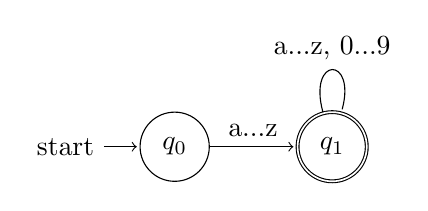
\begin{tikzpicture}[shorten >=1pt, node distance=2cm, on grid, auto]
   \node[state, initial] (q0) {$q_0$};
   \node[state, accepting, right=of q0] (q1) {$q_1$};
   
   \draw[->] (q0) to node {a...z} (q1);
   \draw[loop above] (q1) to node {a...z, 0...9} (q1);
\end{tikzpicture}
\end{center}
\caption{식별자 오토마타}
\label{fig:identifierautumatagraph}
\end{figure}

이 그래프에서 노드는 상태를, 에지는 상태 전이를 나타낸다. 상태 $q_0$는
시작 상태이고 영문자 $a$부터 $z$ 중 하나를 입력 받으면 다음 상태
$q_1$으로 바꾼다. 상태 $q_1$은 종료 상태로 한 개의 영문자가 유효한
식별자로 받아 들인다. 종료 상태는 두 개의 원을 겹쳐서 표시한다. 상태
$q_1$에서 입력이 끝나지 않고 숫자나 영문자가 반복해서 들어와도 누적된
입력을 유효한 식별자로 받아들인다.

이 오토마타는 결정적이다.  모든 상태에서 주어진 어떤 입력에 대해서도
오직 한 가지 방법으로만 상태 전이가 발생하기 때문이다.

또한 이 예시는 다루는 상태의 수가 유한한 유한 오토마타(finite
automata)이다. 상태가 유한하기 때문에 이 오토마타로 다룰 수 있는
정보가 제한적이다.


이 그래프를 함수 $\delta_{id}$로 표시하면 다음과 같다.

\begin{center}
  $\delta_{id}(q_0, a) = q_1$ \\
  ... \\
  $\delta_{id}(q_0, z) = q_1$ \\
  $\delta_{id}(q_1, a) = q_1$ \\
  ... \\
  $\delta_{id}(q_1, z) = q_1$ \\
  $\delta_{id}(q_1, 0) = q_1$ \\
  ... \\
  $\delta_{id}(q_1, 9) = q_1$ \\
\end{center}

(결정적 유한) 오토마타 $M$은 일반적으로 상태 집합 $Q$, 입력 알파벳
기호 $\Sigma$, 전이 함수 $\delta$, 시작 상태 $q_0$, 종료 상태들 $F$,
다섯 가지 구성 요소로 기술한다.


식별자를 인식하는 오토마타 $M_{id}$는 다음과 같이 작성할 수 있다.
\[
M_{id} \ = \ (\{q_0,q_1\}, \ \{a,...,z,0,...9\}, \ \delta_{id}, \ q_0, \ \{q_1\} )
\]

앞서 \ref{subsec:grammar} 장에서 다룬 문법 $G_{id}$에서 만들 수 있는
모든 식별자를 이 오토마타 $M_{id}$에서 유효하다고 판단할까? 반대로 이
오토마타 $M_{id}$에서 유효하다고 판단하는 모든 식별자를 문법
$L_{id}$에서 만들 수 있을까? 두 질문에 대한 답은 그렇다이다.
%
이런 점에서 문법(으로 만들 수 있는 언어)과 오토마타(로 인식할 수 있는
언어)는 동일하다고 한다.
\begin{equation}
  L(M_{id}) \ = \ L(G_{id})
  \label{equ:midisequaltogid}
\end{equation}

식 \ref{equ:gidisequaltolid}과 식 \ref{equ:midisequaltogid}를 조합하면
식별자에 관한 언어와 문법과 오토마타, 세 가지가 모두 동일하다.


\begin{equation}
  L_{id} \ = \ L(G_{id}) \ = \ L(M_{id})
  \label{equ:lisisequaltomidisequaltogid}
\end{equation}

\section{어휘 분석}

어휘 분석은 텍스트를 입력 받아 어휘 명세에 따라 정의된 토큰으로
분리하여 그 토킨 리스트를 출력한다. 예를 들어 그림
\ref{fig:factorial}의 프로그램 텍스트를 입력으로 가정하자.  1과 2번
라인은 다음과 같은 텍스트 문자들로 구성되어 있다.

\begin{center}
  `i', `n', `t', ` ', `x', `;', `\textbackslash n', `i', `n', `t', ` ', `z', `;', `\textbackslash n', ...
\end{center}

어휘 분석을 거치면 아래의 토큰 리스트를 출력한다.

{\small
\begin{center}
  TkTyInt, TkIdentifier ``x'', TkSemiColon, TkTyInt, TkIdentifier ``z'', TkSemiColon, ...
\end{center}
}

WHILE 언어에서 필요한 어휘 또는 토큰은 그림
\ref{fig:haskelltokendatatype}와 같이 정의할 수 있다.

\begin{figure}[h]
{\footnotesize
\begin{center}
\begin{minipage}[h]{.7\textwidth}
\begin{lstlisting}[language=Haskell]
data Token =
    TkEndOfTokens
  | TkCInt         -- 1, 2, 3
  | TkCBool        -- true, false
  | TkIdentifier   -- x, y, abc123, _z
  | TkTyInt        -- int
  | TkTyBool       -- bool
  | TkAdd                 -- +
  | TkSub                 -- -
  | TkMul                 -- *
  | TkDiv                 -- /
  | TkMod                 -- %
  | TkLessThan            -- <
  | TkGreaterThan         -- >
  | TkLessThanEqualTo     -- <=
  | TkGreaterThanEqualTo  -- >=
  | TkEqualTo             -- ==
  | TkNotEqualTo          -- !=
  | TkAnd                 -- &&
  | TkOr                  -- ||
  | TkNot                 -- !
  | TkSkip                -- skip (keyword)
  | TkSemicolon           -- ;
  | TkAssign              -- =
  | TkRead                -- read (keyword)
  | TkWrite               -- write (keyword)
  | TkIf                  -- if (keyword)
  | TkThen                -- then (keyword)
  | TkElse                -- else (keyword)
  | TkWhile               -- while (keyword)
  | TkOpenBrace           -- {
  | TkCloseBrace          -- }
  | TkOpenParen           -- (
  | TkCloseParen          -- )
  | TkAssert              -- assert (keyword)
\end{lstlisting}
\end{minipage}
\end{center}
}
\caption{WHILE 프로그래밍 언어의 토큰 정의 (하스켈로 작성한 명세)}
\label{fig:haskelltokendatatype}
\end{figure}

어휘 분석기는 정규식과 매칭되는 토큰의 쌍을 나열하는 것으로 명세를
작성한다. 예를 들어, WHILE 언어의 어휘 분석기의 일부를 살펴보자.

\begin{center}
\begin{minipage}[h]{.7\textwidth}
  \begin{lstlisting}{language=Haskell}
    [
      ("int", return TkTyInt ),
      (";", return TkSemicolon ),
      ("[_a-zA-Z][a-zA-Z0-9]*", return TkIdentifier ),
      ...
    ]
  \end{lstlisting}
\end{minipage}
\end{center}

\section{구문 구조 분석}

\chapter{의미 분석(Static and dynamis semantics)}

\chapter{정적 프로그램 분석(Static program analysis)}

정적 프로그램 분석은 프로그램 소스를 입력으로 사용하여, 해당 프로그램
실행 시 발생할 수 있는 동작이나 결과 값을 컴파일 시점에서 안전하고
계산 가능한 방법으로 근사치를 예측하는 기술입니다.


이 장에서는 정적 프로그램 분석의 여러 접근 방식 중에서 자료 흐름 분석,
제약식 기반 분석, 요약 해석을 살펴봅니다.

\section{개요}

정적 프로그램 분석을 통해 실행 시 발생할 수 있는 모든 동작과 결과 값을
사전에 예측할 수 있습니다. 이를 통해 프로그램이 의도치 않게 동작하는
상황을 예방할 수 있고, 컴파일러는 실행 속도가 빠르거나 메모리 사용을
최적화한 코드를 생성할 수 있습니다.

도달 가능한 정의 분석(Reaching definitions anlaysis)을 통해 초기화하지
않은 변수를 사용하려는 코드가 있는지 미리 점검할 수 있습니다.
%
사용 가능한 식 분석(Available expressions analysis)을 통해 이미
계산해놓은 결과를 재활용하여 동일한 식을 반복해서 계산하지 않는지
점검할 수 있습니다.
%
루프 내 불변 연산 검출 분석(Loop-invariant computations detection
analysis)을 통해 반복문이 실행되는 동안 항상 동일한 값을 내는 식을
찾을 수 있습니다. 반복문 밖에서 한번만 계산하도록 최적화하는데 사용될
수 있다.

정적 프로그램 분석은 다양한 접근 방법이 있다. 자료 흐름 분석(Data flow
analysis), 제약식 분석(Constraint-based analysis), 요약 해석(Abstract
interpretation), 타입과 효과 시스템(Type and effect systems), 네 가지
대표적인 방법론이 있다.
%
자료 흐름 분석은 G. Kildall이 제안한 공통
프레임워크\cite{kildall1973}에 의한 분석 방법들을 일컫는다. 프로그램을
그래프로 표현하고 노드마다 들어오는 분석 정보를 이용하여 나가는 분석
정보를 계산하는 함수를 정의하여 분석 방법을 정의한다.
%
제약식 분석은 제어 흐름 분석(Control-flow analysis)을 가리킨다. 제어
흐름 분석은 어떤 기본 블록 다음에 실행할 수 있는 기본 블록들 정보를
찾는 방법이다. WHILE 언어 프로그램의 경우 제어 흐름 분석이 간단하지만
함수형 언어 프로그램이나 객체지향 언어 프로그램의 경우 복잡하다.
%
요약 해석은 정적 분석을 유도하는 일반적인 방법론이다. 분석 방법을 먼저
정의하고 그 다음에 이 방법이 유효한가를 확인하는 기존의 방법과 달리
프로그램의 동적 의미를 요약하여 정적 분석 방법을 이끌어내는 방법이다.
%
타입과 효과 시스템은 프로그램의 정적 의미인 타입시스템을 분석하고자
성질에 필요한 요소로 확장하고 타입 검사 방법으로 타입 일관성을 확인할
뿐만 아니라 아니라 프로그램 성질을 분석한다.

이와 같이 정적 분석에 대한 여러 다른 접근 방법이 있지만 모든 정적 분석
방법들은 공통점을 지닌다. 정적 분석 방법은 프로그램을 입력으로 받아
분석 결과를 내고 종료해야한다. 무한히 계산하지 않고 반드시
종료해야하므로 정확히 분석하기보다 안전하고 정밀한 근사치를 내는데
중점을 둔다. 분석 결과는 근사치이다. 즉, 실제로 얻을 수 있지 않은
결과도 포함시킬 수 있다. 하지만 안전한 결과이어야 한다. 즉, 실제로
얻을 수 있는 결과는 모두 포함해야 한다.

\section{자료 흐름 분석}

\section{제약식 분석}

\section{요약 해석}

\chapter{기호 실행}

\chapter{맺음말}


\bibliographystyle{plain}
\bibliography{sav}

\end{document}
